\documentclass[14 pt]{extarticle}

	\usepackage[frenchb]{babel}
	\usepackage[utf8]{inputenc}  
	\usepackage[T1]{fontenc}
	\usepackage{amssymb}
	\usepackage[mathscr]{euscript}
	\usepackage{stmaryrd}
	\usepackage{amsmath}
	\usepackage{tikz}
	\usepackage[all,cmtip]{xy}
	\usepackage{amsthm}
	\usepackage{varioref}
	\usepackage{geometry}
	\geometry{a4paper}
	\usepackage{lmodern}
	\usepackage{hyperref}
	\usepackage{array}
	 \usepackage{fancyhdr}
	 \usepackage{float}
\renewcommand{\theenumi}{\alph{enumi})}
	\pagestyle{fancy}
	\theoremstyle{plain}
	\fancyfoot[C]{} 
	\fancyhead[L]{Contrôle}
	\fancyhead[R]{14 octobre 2022}\geometry{
 a4paper,
 total={170mm,257mm},
 left=20mm,
 top=20mm,
 }
	
	
	\title{Contrôle Chapitre 2}
	\date{}
	\begin{document}

\begin{center}{\Large Contrôle Chapitre 2}\\ 
 \end{center}
 Nom : \\
 Prénom : \\
 \subsection*{Exercice 1 (4 points)}
 
 1) Rappelez la définition de la médiatrice d'un segment $[AB]$. 
 
 2) Recopiez et complétez : Si les points $A$ et $B$ sont symétriques par rapport à la droite $(d)$, alors $(d)$ est la \ldots du \ldots $[AB]$. 
 \subsection*{Exercice 2 (7 points)}
 
 Tracez les symétriques de la figure suivante par rapport à la droite $(d)$ et au point $B$. 
 
 \begin{figure}[H]
 \center
 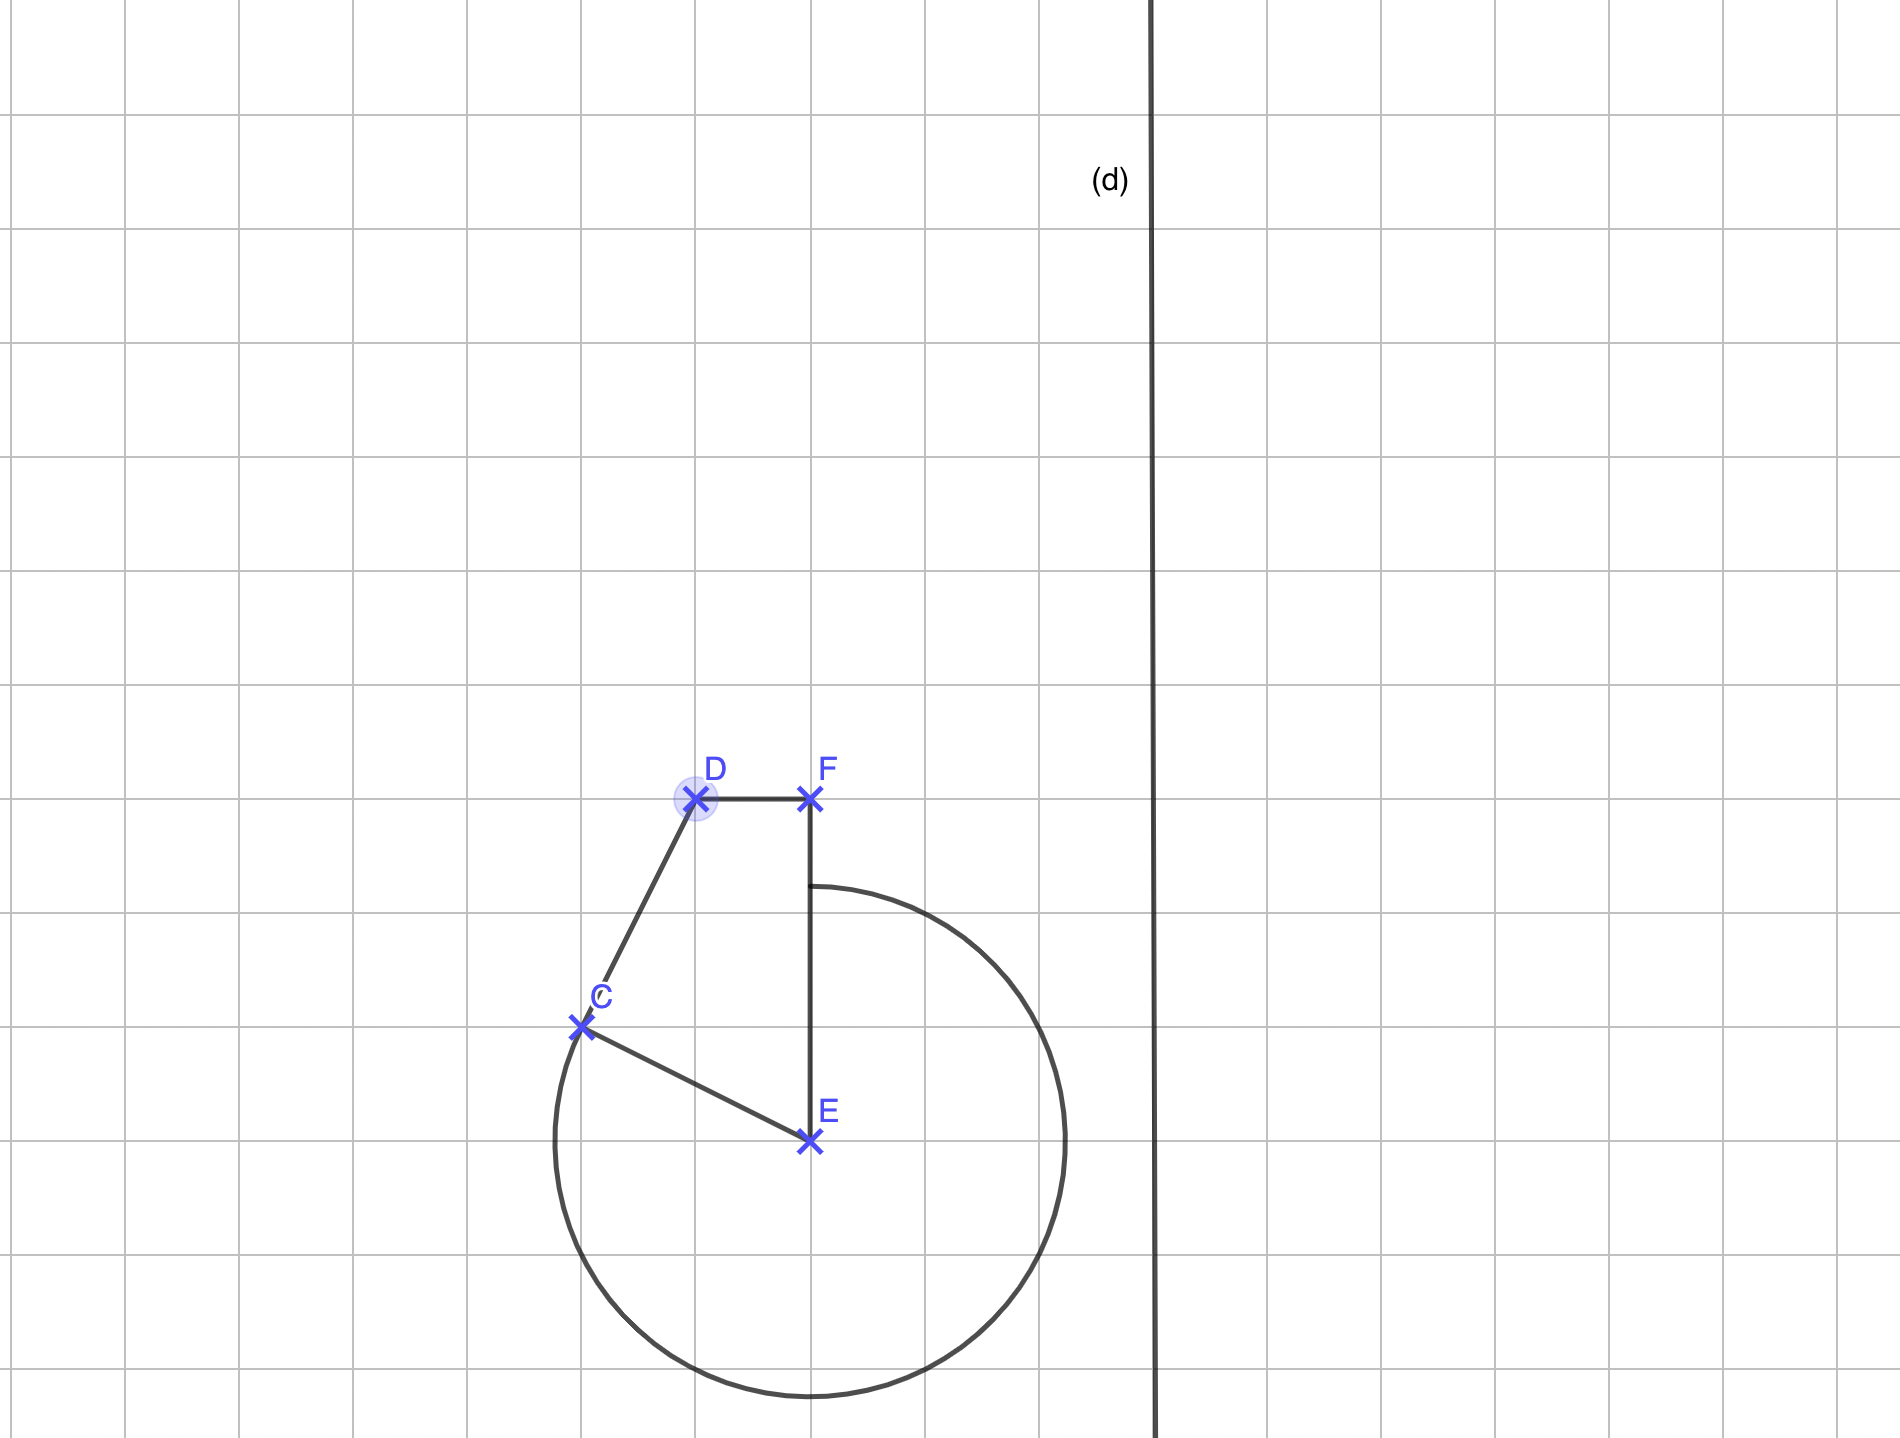
\includegraphics[scale=.55]{Exo1b.png}
 \end{figure}
 
 \subsection*{Exercice 3 (3 points)}
 
 \begin{enumerate}
 \item Tracez un rectangle de côtés $4$ cm et $6$ cm. 
 \item Combien a-t-il d'axes de symétrie ? Tracez-les sur la figure.
 \item A-t-il un centre de symétrie ? Si oui, le représenter sur la
 figure. 
 \end{enumerate}
 
\subsection*{Exercice 4 (3 points)} 

Sur les figures suivantes, représentez les axes et centres de symétrie éventuels, et dites leur nombre.  

\begin{figure}[H]
\center 

\includegraphics[scale=.06]{ecosse.png}\ \ \ \ \ 

\includegraphics[scale=.6]{Blason2.png}\ \ \ \ \ 
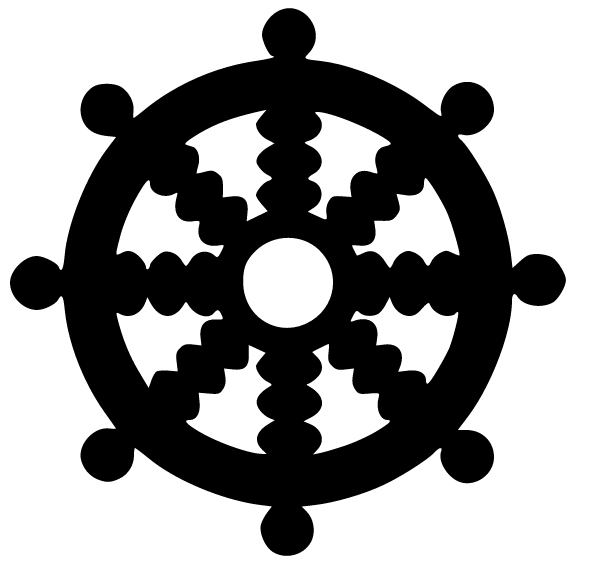
\includegraphics[scale=.4]{Symb2.png}
\end{figure}
 
 \subsection*{Exercice 5 (3 points au moins)}
 
On veut montrer qu'un quadrilatère dont les diagonales sont des axes de symétrie est un losange. On prend donc un quadrilatère $ABCD$, et on suppose que $(AC)$ et $(BD)$ sont des axes de symétrie. 

\begin{enumerate}
\item Faire une figure à main levée.
\item Quel est le symétrique du point $B$ par rapport à $(AC)$ ?  
\item En déduire que les segments $[AB]$ et $[AD]$ sont symétriques 
par rapport à la droite $(AC)$. 
\item En déduire que $AB=AD$. 
\item Montrer de la même manière que $CB = CD$. 
\item En utilisant cette fois la symétrie par rapport à $(BD)$, 
montrer que $AB=BC$. 
\item Justifier que $ABCD$ est un losange. 
\end{enumerate}







 	\end{document}
